\documentclass[12pt, a4paper, twoside]{article}
\usepackage[left = 3cm, top = 3cm, right = 2cm, bottom = 2cm]{geometry}
\usepackage[brazilian]{babel}
\usepackage[utf8]{inputenc}
\usepackage{amsmath, amsfonts, amssymb, amsthm}
\numberwithin{equation}{subsection} %subsection
\usepackage{fancyhdr}
\usepackage{graphicx}
\usepackage{colortbl}
\usepackage{titletoc,titlesec}
\usepackage{setspace}
\usepackage{indentfirst}
%\usepackage{natbib}
\usepackage[colorlinks=true, allcolors=black]{hyperref}
%\usepackage[brazilian,hyperpageref]{backref}
\usepackage[alf]{abntex2cite}
\usepackage{multirow} % https://www.ctan.org/pkg/multirow
\usepackage{float} % https://www.ctan.org/pkg/float
\usepackage{booktabs} % https://www.ctan.org/pkg/booktabs
\usepackage{enumitem} % https://www.ctan.org/pkg/enumitem
\usepackage{quoting} % https://www.ctan.org/pkg/quoting
\usepackage{epigraph}
\usepackage{subfigure}
\usepackage{anyfontsize}
\usepackage{caption}
\usepackage{adjustbox}
\usepackage{bm}
%\usepackage{tocbibind}
\usepackage[titletoc,page]{appendix}
\usepackage{hyperref}
\usepackage{fancyhdr}
\usepackage{multicol}
\usepackage{pgf}
\usepackage{refcount}
\usepackage{xfp}
\usepackage{newfloat}
\usepackage{caption}
\usepackage{tikz}

% Define o novo ambiente flutuante "Modelo"
\DeclareFloatingEnvironment[
    fileext=lod,
    listname=Lista de Modelos,
    name=Modelo,
    placement=tbhp,
]{modelo}

\newcommand{\calcref}[2]{\fpeval{#1-#2}}

\def\checkmark{\tikz\fill[scale=0.4](0,.35) -- (.25,0) -- (1,.7) -- (.25,.15) -- cycle;} 


%\usepackage[style=abnt]{biblatex}
%\bibliographystyle{plainnat}
\raggedbottom % https://latexref.xyz/_005craggedbottom.html

\newtheorem{teo}{Teorema}[section]
\newtheorem{lema}[teo]{Lema}
\newtheorem{cor}[teo]{Corolário}
\newtheorem{prop}[teo]{Proposição}
\newtheorem{defi}{Definição}
\newtheorem{exem}{Exemplo}

\newcommand{\titulo}{Determinantes do tempo até a baixa de processos \\ na Justiça do Trabalho}
\newcommand{\autor}{Kassyano Kevyn Andrade de Souza}
\newcommand{\orientador}{ Thais Carvalho Valadares Rodrigues }

\pagestyle{fancy}
\fancyhf{}
%\renewcommand{\headrulewidth}{0pt}
\setlength{\headheight}{16pt}
%C - Centro, L - Esquerda, R - Direita, O - impar, E - par
\fancyhead[RO, LE]{\thepage}
\renewcommand{\sectionmark}[1]{\markboth{#1}{}}

\titlecontents{section}[0cm]{}{\bf\thecontentslabel\ }{}{\titlerule*[.75pc]{.}\contentspage}
\titlecontents{subsection}[0.75cm]{}{\thecontentslabel\ }{}{\titlerule*[.75pc]{.}\contentspage}

\setcounter{secnumdepth}{3}
%\setcounter{tocdepth}{3}

\DeclareCaptionFormat{myformat}{ \centering \fontsize{10}{12}\selectfont#1#2#3}
\captionsetup{format=myformat}

\begin{document}


\begin{titlepage}
\begin{center}
\begin{figure}[h!]
	\centering
		
\includegraphics[scale = 0.095]{imagens/unb.pdf}
            %
\includegraphics[scale = 0.8]{imagens/unb.png}
	\label{fig:unb}
\end{figure}
{\bf Universidade de Brasília \\
\bf Departamento de Estatística}
\vspace{5cm}

\setcounter{page}{0}
\null
\textbf{\titulo}
\vspace{2.5cm}


\vspace{0.2cm}
\textbf{\autor}
\end{center}
\vspace{1.5cm}

\begin{flushright}
\begin{minipage}{7.5cm}
\parbox[t]{7.5cm}{Projeto apresentado para o Departamento de Estatística da Universidade de Brasília como parte dos requisitos necessários para obtenção do grau de Bacharel em Estatística.}
\end{minipage}
\end{flushright}

\vspace{5cm}

\begin{center}
{\bf{Brasília} \\ }
\bf{2023}
\end{center}

\end{titlepage}


\thispagestyle{empty}

\begin{center}
\textbf{\autor} \\
\vspace{5cm}
\textbf{\titulo} \\
\vspace{3cm}
\small
Orientador(a): \orientador \\
Coorientador(a): \coorientador
\end{center}


\vspace*{3cm}

\begin{flushright}
\begin{minipage}{7.5cm}
 \parbox[t]{7.5cm}{Projeto apresentado para o Departamento de Estatística da Universidade de Brasília como parte dos requisitos necessários para obtenção do grau de Bacharel em Estatística.}
\end{minipage}
\end{flushright}

\vspace{5cm}

\begin{center}
{\bf{Brasília} \\ }
\bf{2023}
\end{center}




\pagenumbering{gobble}
%\setcounter{page}{2}
\onehalfspacing




\setlength{\parindent}{1.5cm}
\setlength{\parskip}{0.2cm}
\setlength{\intextsep}{0.5cm}

\titlespacing*{\section}{0cm}{0cm}{0.5cm}
\titlespacing*{\subsection}{0cm}{0.5cm}{0.5cm}
\titlespacing*{\subsubsection}{0cm}{0.5cm}{0.5cm}
\titlespacing*{\paragraph}{0cm}{0.5cm}{0.5cm}

\titleformat{\paragraph}
{\normalfont\normalsize\bfseries}{\theparagraph}{1em}{}
%\titlespacing*{\paragraph}
%{0pt}{3.25ex plus ex minus .2ex}{1.5ex plus .2ex}





\fancyhead[RE, LO]{\nouppercase{\emph\leftmark}}
%\fancyfoot[C]{Departamento de Estatística}

%%%%%%%%%%%%%%%%%%%%%%%%%%%%%%%%%%%%%%%%%%%%%%%%%%%%%%%%%%%%%%%%%%%%%%%%%%%%%%%%%%%%%%%%%%%%%%%%%%%%%%%%%%
%%%%%%%%%%%%%%%%%%%%%%%%%%%%%%%%		Dedicatória			%%%%%%%%%%%%%%%%%%%%%%%%%%%%%%%%%%%%%%%%%%%%%%
%%%%%%%%%%%%%%%%%%%%%%%%%%%%%%%%%%%%%%%%%%%%%%%%%%%%%%%%%%%%%%%%%%%%%%%%%%%%%%%%%%%%%%%%%%%%%%%%%%%%%%%%%%

%``exemplo"

\vspace*{13cm}

\hfill{\begin{minipage}{10.4cm}
\textit{Dedico este trabalho à classe operária, que tem na venda de sua força de trabalho o único meio de garantir a sua sobrevivência, mas cujo trabalho é o que garante a nossa própria existência.}

\end{minipage}}
\newpage

%%%%%%%%%%%%%%%%%%%%%%%%%%%%%%%%%%%%%%%%%%%%%%%%%%%%%%%%%%%%%%%%%%%%%%%%%%%%%%%%%%%%%%%%%%%%%%%%%%%%%%%%%%
%%%%%%%%%%%%%%%%%%%%%%%%%%%%%%%%		Agradecimentos			%%%%%%%%%%%%%%%%%%%%%%%%%%%%%%%%%%%%%%%%%%
%%%%%%%%%%%%%%%%%%%%%%%%%%%%%%%%%%%%%%%%%%%%%%%%%%%%%%%%%%%%%%%%%%%%%%%%%%%%%%%%%%%%%%%%%%%%%%%%%%%%%%%%%%


\vspace*{2.5cm}

\begin{center}
 {\Huge \bfseries Agradecimentos}
\end{center}
\baselineskip 19.5pt 
\vspace*{1.5cm}

Agradeço à minha ilustre, impecável, incomparável, intransponível e insubstituível orientadora, Thais Rodrigues, por ter me acompanhado e instruído durante todo o projeto.

Aos meus colegas de faculdade e amigos com quem estudei durante os últimos anos, André Vale, Carolina Musso, César Galvão, Davi Guerra, Eduardo Côrtes, Emilly Marques, Hermes Winarski, Juliana Degani, Juliana Rocha, Juliana Rosa, Laura Melo, Matheus Martinez, Maria Luiza Escobar, Micael Papa, Pedro Tepedino, Rafael de Acypreste, a recém-chegada Rita Veloso, Sabrina França, Silvânia Andrade e Tamara Dias, agradeço por fazerem parte da minha vida. A experiência da universidade, tampouco a experiência da própria vida, jamais teria sido a mesma sem vocês.

Aos meus amigos de longa data, Ana Lúcia Amado, Camylla Meirelly, Daniel Badaró, Fernanda Gomes, Gabriel Machado, Hudson Pimenta, Letícia Pimenta, Rodrigo de Carvalho, Rodrigo de Freitas, Samuel Barbosa, Silas Bismarck e Tatianne Gomes, agradeço por estarem comigo nos comigo nos piores momentos e terem me incentivado constantemente a seguir os meus sonhos. Ao meu amigo, Lourival Silva,     eternizo sua memória com este agradecimento póstumo.

Aos meus colegas do Eixo 4, Ana Rezende, Carlos Becker, Genesis Pereira, Igor Stemler, Isabely Mota, Rayssa Coátio, Ricardo Guidoni e Viviane Fecher, agradeço por terem me incentivado e ajudado a compreender os dados com os quais trabalhei nesse projeto. 

Agradeço aos meus webamigos Eduardo Moreira (EliminatorVenom/BLU Spy), Lucas Silva (DeusDoMalDDM), Matheus Rabelo (Takato Blue) e Vinnie Quintana, pelos mais de 10 anos nos quais no conhecemos, e por todas as fases que atravessamos nesse webmundo. A presença de vocês para mim é tão real quanto toda a realidade que me cerca.

Agradeço à minha cachorra, Gabi, e ao meu gato, Thomas, embora o fato de que eles ainda não chegaram à idade de aprender a ler os impeça de tomarem ciência deste agradecimento.

À minha mãe, Neuza Andrade, e meu pai, Gilmar Souza, agradeço por todo o apoio que me deram para que eu pudesse chegar até aqui.

Por fim, a cada Kevyn dos outros infinitos mundos possíveis (exceto os maus) que seguiram por caminhos diferentes do meu, agradeço pela perseverança. Espero que tenham superado o sofrimento sutil da impermanência e a insatisfação inerente à existência, e encontrado a paz em seus caminhos.

\newpage

%%%%%%%%%%%%%%%%%%%%%%%%%%%%%%%%%%%%%%%%%%%%%%%%%%%%%%%%%%%%%%%%%%%%%%%%%%%%%%%%%%%%%%%%%%%%%%%%%%%%%%%%%%
%%%%%%%%%%%%%%%%%%%%%%%%%%%%%%%%%%%%		Resumo			%%%%%%%%%%%%%%%%%%%%%%%%%%%%%%%%%%%%%%%%%%%%%%
%%%%%%%%%%%%%%%%%%%%%%%%%%%%%%%%%%%%%%%%%%%%%%%%%%%%%%%%%%%%%%%%%%%%%%%%%%%%%%%%%%%%%%%%%%%%%%%%%%%%%%%%%%

%\vspace*{2.5cm}
%\begin{center}
% {\Huge \bfseries Resumo}
%\end{center}
%\baselineskip 19.5pt 
%\vspace*{1.5cm}
%
%Texto...
%
%\vspace*{1.5cm}
%
%Palavras-chaves: 

  
\newpage


%%%%%%%%%%%%%%%%%%%%%%%%%%%%%%%%%%%%%%%%%%%%%%%%%%%%%%%%%%%%%%%%%%%%%%%%%%%%%%%%%%%%%%%%%%%%%%%%%%%%%%%%%%
%%%%%%%%%%%%%%%%%%%%%%%%%%%%%%%%		Tabelas/Figuras			%%%%%%%%%%%%%%%%%%%%%%%%%%%%%%%%%%%%%%%%%%
%%%%%%%%%%%%%%%%%%%%%%%%%%%%%%%%%%%%%%%%%%%%%%%%%%%%%%%%%%%%%%%%%%%%%%%%%%%%%%%%%%%%%%%%%%%%%%%%%%%%%%%%%%

\listoftables

\newpage

\listoffigures

\newpage

\listofmodelo

\newpage
%Sumário
\tableofcontents

\newpage

\pagenumbering{arabic}
\setcounter{page}{8}

\section{\textbf{Introdução}}
O Poder Judiciário é um dos poderes fundamentais da estrutura tripartite do Estado brasileiro. Suas ações estão diretamente atreladas ao funcionamento das instituições de Estado e à manutenção da justiça, suscitando interesse para a administração pública. O entendimento da dinâmica judicial é o que garante sua transparência e credibilidade frente à sociedade civil.

Nos últimos anos, o emprego de tecnologias para aumento de eficiência dos serviços prestados tem sido uma preocupação do Poder Judiciário, e o Conselho Nacional de Justiça (CNJ) tem proposto medidas para cumprir esse fim, tais como o Processo Judicial Eletrônico \cite{pje} e o Juízo 100\% Digital \cite{juizo100digital}.

O Relatório Justiça em Números, que publica anualmente estatísticas sobre o Poder Judiciário, mostrou que, em 2021, o Brasil detinha uma relação de 8,5 magistrados para cada 100.000 habitantes, que configura aproximadamente metade do valor relativo na comparação com países europeus \cite{justicaemnumeros}. \citeonline{satiro2021desempenho}, ao investigar determinantes da produtividade do Poder Judiciário, concluíram que o número de servidores, advogados, empregados terceirizados e a carga de trabalho têm influência direta na produtividade de um tribunal.

Para este projeto, a principal variável analisada será o tempo compreendido entre o início do processo e sua baixa, que pertence à classe de indicadores de tempo de tramitação. As baixas, por sua vez, são definidas como quaisquer processos que sejam “[...] a) remetidos para outros órgãos judiciais competentes, desde que vinculados a tribunais diferentes; b) remetidos para as instâncias superiores ou inferiores; c) arquivados definitivamente.” \cite{painelestatistica}.

A relevância dessa classe de indicadores se dá pelo fato de que uma baixa configura um encerramento da situação de pendente de um processo. O estudo visa avaliar como esse tempo se distribui entre os órgãos julgadores da Justiça do Trabalho, e quais variáveis podem influenciar em sua redução ou aumento. Tal propósito será cumprido com a construção de um modelo de regressão quantílica. O modelo vai permitir observar quais varas estão abaixo ou acima de determinada faixa, analisar tendências e extrair resultados probabilísticos.



%\citeonline{david2000applied}



\newpage

\section{\textbf{Objetivos}}
\subsection{Objetivo Geral}
O objetivo deste trabalho é estudar o tempo até a baixa de processos no ramo da Justiça do Trabalho, utilizando dados do Poder Judiciário Brasileiro no retrato referente a janeiro de 2024, e descrever como ele se distribui com relação às características da vara, de forma que seja possível predizer esse tempo dadas as covariáveis disponíveis.

\subsection{Objetivos Específicos}

\begin{itemize}
    \item Estudar a regressão quantílica e seu impacto no estudo da produtividade dos tribunais da Justiça do Trabalho;
    \item Comparar os resultados da regressão quantílica com os resultados da regressão tradicional para a média;
    \item Estudar as variáveis que impactam no tempo médio entre o início dos processos e suas baixas;
\end{itemize}


\newpage
%\section{\textbf{Justificativa}}
%\input{justificativa.tex}

\newpage

\section{\textbf{Referencial Teórico}}
A análise de regressão é um conjunto de métodos estatísticos que buscam ajustar uma função preditora de uma variável resposta com base em uma ou mais variáveis explicativas.

Seja $X$ uma variável explicativa e $Y$ uma variável resposta. Para cada $X$, deseja-se estimar a distribuição condicional de $Y | X$, conforme ilustrado na Figura \ref{fig:exemplo_regressao}.

\begin{figure}[H]
    \centering
    \caption{Dispersão de pontos com distribuições de $Y | X$}
    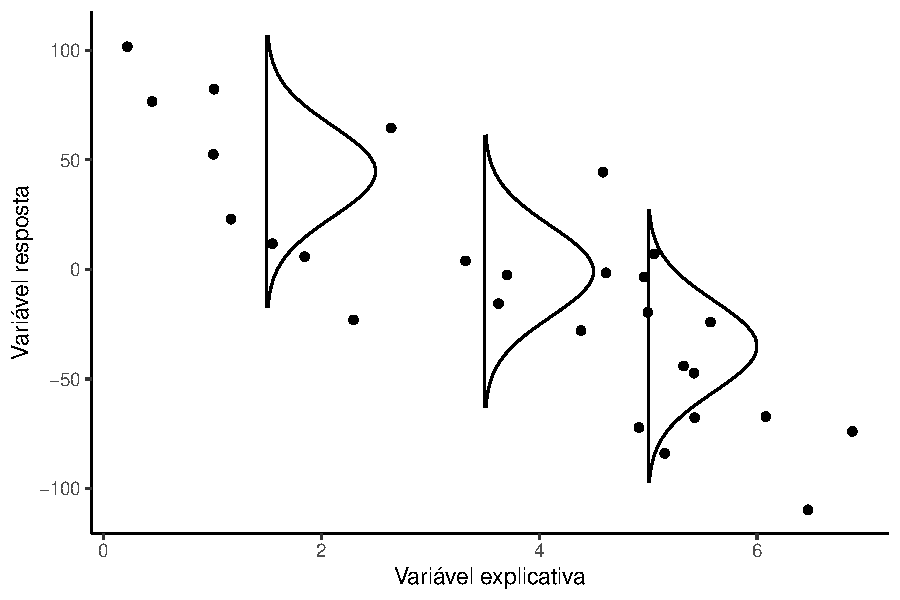
\includegraphics[scale=1.05]{imagens/scatter2.pdf}
    \label{fig:exemplo_regressao}
\end{figure}

 Os dois métodos que serão utilizados no trabalho, cujos resultados serão comparados entre eles, são a regressão gaussiana e a regressão quantílica, que estimam, respectivamente, a média condicional $E(Y|X)$ e os quantis condicionais $Q(Y|X)_\tau$.

\subsection{Regressão Gaussiana}
A regressão gaussiana linear, ou regressão tradicional, é um método que ajusta uma reta que minimiza a diferença quadrática entre um conjunto de pontos e a média observada.

Há cinco pressupostos principais para um modelo de regressão gaussiana:

\begin{enumerate}
    \item A correlação entre a média condicional E(Y|X) da variável resposta e as variáveis explicativas é linear, ou seja, descrita por uma combinação linear entre as variáveis explicativas e os parâmetros do modelo.
    \item Os erros $\varepsilon_i$ tem média $\mu = 0$.
    \item Os erros $\varepsilon_i$ tem variância constante $\sigma^2$.
    \item Os erros $\varepsilon_i$ são não-correlacionados entre eles.
    \item Os erros possuem distribuição Normal.
\end{enumerate}

Seja $\mathbf{x}$ um vetor de variáveis aleatórias independentes e $\varepsilon$ um vetor de erros aleatórios, onde $\varepsilon$ satisfaz a propriedade de ser Normalmente distribuído, com média $\mu = 0$ e variância $\sigma_i ^ 2$ constante para cada $\varepsilon_i$, qualquer que seja o valor de $x_i$ ($i \in \{1, \dots, n\}$). Seja $Y$ uma variável resposta. A regressão gaussiana ajusta um vetor de coeficientes $\beta$ de uma equação
\begin{equation}
Y = \beta ^ {T} \mathbf{x} + \varepsilon,
\end{equation}

\noindent minimizando a soma dos quadrados dos erros, e prediz o valor médio de $Y$ condicionado aos valores de $\mathbf{x}$.

É possível demonstrar que, satisfeitos os pressupostos do modelo, o vetor de coeficientes $\beta$ pode ser estimado na forma

\begin{equation}
\hat{\beta} = (\mathbf{X}^{T}\mathbf{X})^{-1} \mathbf{X}^{T} \mathbf{y},
\end{equation}

\noindent onde $\mathbf{X}$ é a matriz de valores observados ordenados das variáveis explicativas, e $\mathbf{y}$ é o vetor de valores observados da variável resposta $Y$ \cite{montgomerylra}.

\newpage
\subsection{Regressão Quantílica}
No que se refere aos pressupostos, a regressão quantílica é menos restritiva do que o modelo gaussiano, pois não assume Normalidade dos erros, tampouco homoscedasticidade. A regressão quantílica assume que os erros são não-correlacionados entre eles e $Q_\tau(\varepsilon_\tau | x) = 0$.

Embora modelos quantílicos não-lineares também sejam possíveis, este projeto assumirá que as relações entre as variáveis são lineares.

Diferente do modelo de regressão gaussiana, que traça a reta para a média de uma variável resposta dependente de variáveis explicativas, a regressão quantílica traça a reta para qualquer quantil selecionado. Isso a torna mais robusta que o modelo de mínimos quadrados no que se refere à influência de outliers. Assim, é possível obter análises mais ricas sobre o fenômeno estudado, expandindo a funcionalidade clássica dos modelos de regressão.

O $\tau$-ésimo quantil de uma distribuição de probabilidades é qualquer ponto $y$ da variável aleatória tal que a probabilidade de um valor ser menor ou igual a $y$ é igual a $\tau$. Pela definição, considerando $F(y)$ a função de distribuição acumulada da variável aleatória $y$, temos que

\begin{equation}
\tau = P(Y \leq y) = F(y).
\end{equation}

No caso empírico, com probabilidades zeradas no intervalo entre duas observações, convenciona-se o uso do valor mínimo do intervalo, de modo que a definição para o quantil assume a forma
\begin{equation}
F^{-1}(\tau) = \text{inf}\{y: F(y) \geq \tau\}.
\end{equation}

A distribuição empírica permite reduzir a estimativa para o quantil segundo métodos de otimização da função de perda

\begin{equation}
\rho_\tau(u) = u(\tau - I(u < 0)), \tau \in (0, 1),
\end{equation}

\noindent onde $I(u < 0)$ é uma função indicadora que assume valor 1 se $u < 0$ e valor 0, caso contrário. Os métodos de otimização podem ser implementados computacionalmente com programação linear. Assim, encontra-se o $\hat{x}$ que minimiza

\begin{equation}
\displaystyle \min_{\xi \in \mathbb{R}} \displaystyle \sum_{i=1}^{n} \rho_\tau(y_i - \xi).
\end{equation}

Analogamente, podemos reduzir o problema da regressão quantílica a um problema de otimização de uma distribuição condicional. Segue que o resultado deve resolver

\begin{equation}
\displaystyle \min_{\beta \in \mathbb{R}^{p}} \displaystyle \sum_{i=1}^{n} \rho_\tau(y_i - x_i^{\text{T}}\beta).
\end{equation}


Seja $Q_\tau(Y | X)$ a função de quantil condicional, com Y sendo uma variável aleatória dependente e X conhecido. Seja $\beta$ um vetor de funções de $\tau$ que multiplicam as variáveis explicativas. É possível demonstrar que, resolvido o problema de otimização, obtém-se uma expressão da forma

\begin{equation}
Q_\tau(Y | X) = \beta_0(\tau) + x_1 \beta_1(\tau) + \dots + x_n \beta_n(\tau)  = {\beta} (\tau) \mathbf{x}
\end{equation}

\noindent onde cada $x_{i}$, com $i \in \{1, ..., n\}$, é uma variável explicativa, e $Q_\tau(Y | X)$ é o quantil condicional $\tau$ de $Y$ dado $X$  \cite{koenker2005}.

Se a variação do $\beta(\tau)$ for pequena em função de $\tau$, significa que os erros são identicamente distribuídos, tornando a abordagem de regressão quantílica desnecessária, uma vez que a mesma solução poderia ser modelada a partir de uma regressão linear clássica usando menos recurso computacional. A abordagem quantílica, portanto, se torna faz mais necessária em casos heteroscedásticos, com os quais a regressão linear não teria seus pressupostos satisfeitos.

\subsubsection{Intervalos de confiança para os coeficientes do modelo de regressão quantílica}
A construção de intervalos de confiança será utilizada na 

\newpage



\section{\textbf{Metodologia}}

\subsection{Conjunto de dados}

A Base Nacional de Dados do Poder Judiciário (DataJud) é uma fonte primária que centraliza todos os dados referentes a processos judiciais, englobando tanto processos públicos quanto processos sigilosos, bem como físicos e eletrônicos \cite{datajud}. Os dados a serem utilizados neste projeto são todos oriundos do DataJud, dentre os quais a principal fonte será a Tabela Fato, que alimenta o Painel de Estatísticas do Poder Judiciário \cite{painelestatistica}.

Embora o DataJud contenha dados de processos sigilosos, a Tabela Fato agrega esses dados, removendo o nível de processo, de modo que nenhum processo possa ser identificado de forma individual. Esses dados são atualizados constantemente, e disponibilizados publicamente pelo Conselho Nacional de Justiça.

A Tabela Fato utilizada compreende desde o início de 2021 até janeiro de 2024. Todas as análises de evolução de indicadores ao longo do tempo considerarão este período. Todavia, quaisquer avaliações que não envolvam evolução ao longo do tempo considerarão apenas o mês mais recente disponível, que representa as condições do Poder Judiciário no momento em que os dados foram obtidos.

Com o período completo, a tabela para a Justiça do Trabalho possui 566.196 linhas. Filtrando o período para a data mais recente, esse número cai para 14.045 linhas.

Os níveis de agregação da Tabela Fato são:
    
\begin{itemize}
    \item Grau de Jurisdição: Grau em que o processo está ou esteve em tramitação;
    \item Formato: Se físico ou eletrônico;
    \item Procedimento:
    \begin{itemize}
        \item Conhecimento (criminal ou não criminal), onde se coleta e fornece provas ao juiz responsável;
        \item Execução (judicial, fiscal, extrajudicial não fiscal e penal), onde se cumpre uma decisão judicial;
    \end{itemize}
    \item Se originário ou recursal;
    \item Data: Ano e mês em que a situação do processo referente ao indicador em análise estava em tramitação.
\end{itemize}

São disponíveis 26 indicadores para cada um desses níveis de agregação, que mostram: 

\begin{itemize}
    \item o quantitativo de processos em determinada situação naquele período;
    \item as datas referentes a processos (por exemplo, a menor e a maior data dentre os 5\% de processos mais antigos ainda em tramitação);
    \item o tempo compreendido entre uma situação processual e outra.
    
\end{itemize}

Algumas dessas métricas serão usadas para a construção do modelo preditivo. As variáveis explicativas serão as características da vara de justiça e dos processos, tais como grau de jurisdição, quantidade de processos eletrônicos e a quantidade de processos pendentes. A variável resposta, por sua vez, será o indicador agregado de número 16, que representa o tempo médio entre o início do processo e a baixa, em dias. Esse tempo é representado como uma média devido à natureza agregada dos dados. Ao longo do trabalho, essa variável será referenciada como "tempo até a baixa".


\newpage

%\section{\textbf{Cronograma}}
%\begin{multicols}{2}
\begin{enumerate}
	\item \label{etapa1} Escolha do tema a ser abordado.
	\item \label{etapa2} Desenvolvimento da proposta de projeto.
	\item \label{etapa3} Entrega da proposta de projeto.
	\item \label{etapa4} Revisão de literatura.
	\item \label{etapa5} Elaboração da apresentação da proposta.
	\item \label{etapa6}  Apresentação oral da proposta.
	\item \label{etapa7} Manipulação do banco de dados.
	\item \label{etapa8}  Análise exploratória do banco de dados.
	\item \label{etapa9} Elaboração do relatório parcial.
	\item \label{etapa10} Entrega do relatório parcial ao Professor Orientador(a).
	\item \label{etapa11} Correção do do relatório parcial.
	\item \label{etapa12} Entrega do relatório parcial para a banca.
	\item \label{etapa13} Desenvolvimento do modelo.
        \item \label{etapa14} Elaboração do relatório final.
	\item \label{etapa15} Entrega do relatório final ao Professor Orientador(a).
	\item \label{etapa16} Correção do do relatório final.
	\item \label{etapa17} Entrega do relatório final para a banca.
\end{enumerate}
\end{multicols}


\definecolor{midgray}{gray}{.5}
\def\tablename{Tabela }%
\begin{table}[H]\scriptsize
\centering {\caption{Cronograma}
		\begin{tabular}{|c|c|c|c|c|c|c|c|c|c|}
		\hline
		&\multicolumn{4}{c|}{1/2023}&\multicolumn{5}{c|}{2/2023}\\
		\hline
		& Abril & Maio & Junho & Julho & Agosto & Setembro & Outubro & Novembro & Dezembro\\
		\hline
		\ref{etapa1}&\cellcolor{midgray}&&&&&&&&\\
		\hline
		\ref{etapa2}&\cellcolor{midgray}&\cellcolor{midgray}&&&&&&&\\
		\hline	
		\ref{etapa3}&&\cellcolor{midgray}&&&&&&&\\
		\hline			
		\ref{etapa4}&\cellcolor{midgray}&\cellcolor{midgray}&&&&&&&\\
		\hline	
		\ref{etapa5}&\cellcolor{midgray}&\cellcolor{midgray}&&&&&&&\\
		\hline
		\ref{etapa6}&&\cellcolor{midgray}&\cellcolor{midgray}&&&&&&\\
		\hline	
		\ref{etapa7}&&&\cellcolor{midgray}&&&&&&\\
		\hline	
		\ref{etapa8}&&&\cellcolor{midgray}&\cellcolor{midgray}&&&&&\\
		\hline	
		\ref{etapa9}&&&\cellcolor{midgray}&\cellcolor{midgray}&&&&&\\
		\hline	
		\ref{etapa10}&&&&\cellcolor{midgray}&&&&&\\
		\hline	
		\ref{etapa11}&&&&\cellcolor{midgray}&&&&&\\
		\hline	
		\ref{etapa12}&&&&\cellcolor{midgray}&&&&&\\
		\hline	
		\ref{etapa13}&&&&&\cellcolor{midgray}&\cellcolor{midgray}&&&\\
        \hline
        \ref{etapa14}&&&&&\cellcolor{midgray}&\cellcolor{midgray}&\cellcolor{midgray}&&\\
        \hline
        \ref{etapa15}&&&&&&&\cellcolor{midgray}&&\\
        \hline
        \ref{etapa16}&&&&&&&\cellcolor{midgray}&\cellcolor{midgray}&\cellcolor{midgray}\cellcolor{midgray}\\
        \hline	
        \ref{etapa17}&&&&&&&&&\cellcolor{midgray}\\
        \hline
		\end{tabular}}
\end{table}


\newpage
\section{\textbf{Resultados}}
\subsection{Análise exploratória}
\subsubsection{Quantidade de Órgãos Julgadores}

A Tabela \ref{tbl:tribunais_qtd_ojs} exibe a quantidade de órgãos julgadores por tribunal.

\begin{table}[ht]
\centering
\caption{Quantidade de órgãos julgadores por tribunal}
\begin{tabular}{c c|cc}
  \hline
 Tribunal & Estado & Frequência & Porcentagem \\ 
   \hline
  TRT2 & SP & 319 & 14,23\% \\ 
  TRT1 & RJ & 222 & 9,91\% \\ 
  TRT15 & SP & 218 & 9,73\% \\ 
  TRT3 & MG & 210 & 9,37\% \\ 
  TRT4 & RS & 190 & 8,48\% \\ 
  TRT9 & PR & 140 & 6,25\% \\ 
  TRT5 & BA & 111 & 4,95\% \\ 
  TRT6 & PE &  97 & 4,33\% \\ 
  TRT12 & SC &  86 & 3,84\% \\ 
  TRT8 & AP e PA &  77 & 3,44\% \\ 
  TRT18 & GO &  64 & 2,86\% \\ 
  TRT7 & CE &  56 & 2,5\% \\ 
  TRT10 & DF e TO &  55 & 2,45\% \\ 
  TRT11 & AM e RR &  48 & 2,14\% \\ 
  TRT23 & MT &  45 & 2,01\% \\ 
  TRT13 & PB &  43 & 1,92\% \\ 
  TRT14 & AC e RO &  41 & 1,83\% \\ 
  TRT17 & ES &  41 & 1,83\% \\ 
  TRT24 & MS &  39 & 1,74\% \\ 
  TRT21 & RN &  35 & 1,56\% \\ 
  TRT19 & AL &  31 & 1,38\% \\ 
  TRT16 & MA &  26 & 1,16\% \\ 
  TRT22 & PI &  24 & 1,07\% \\ 
  TRT20 & SE &  23 & 1,03\% \\
  \hline
  \textbf{Total} & \textbf{Nacional} & 2.241 & 100\% \\ \hline
\end{tabular}
\label{tbl:tribunais_qtd_ojs}
\end{table}

Dos tribunais trabalhistas, o que conta com maior representação em quantidade de órgãos julgadores é o TRT2, com pouco mais de 13\% do total nacional. Dois dos tribunais trabalhistas com mais órgãos julgadores são pertencentes ao estado de São Paulo, correspondendo, juntos, a quase 25\% do total nacional. O estado de São Paulo é, também, a única unidade federativa com dois tribunais da Justiça do Trabalho.

Há quatro tribunais da Justiça do Trabalho que possuem jurisdição em mais de uma Unidade da Federação (UF): TRT8, TRT10, TRT11 e TRT14. Todos esses se restringem a operar em duas UFs cada.

A diferença entre os tribunais para cada ranking decresce de forma suave, sem nenhum grande salto entre um colocado e seu posterior ou anterior. O ramo trabalhista conta com um total de 2.241 órgãos julgadores.


\subsubsection{Distribuição dos tempos}
\begin{figure}[H]
    \centering
    \caption{Distribuição dos tempos até a baixa}
    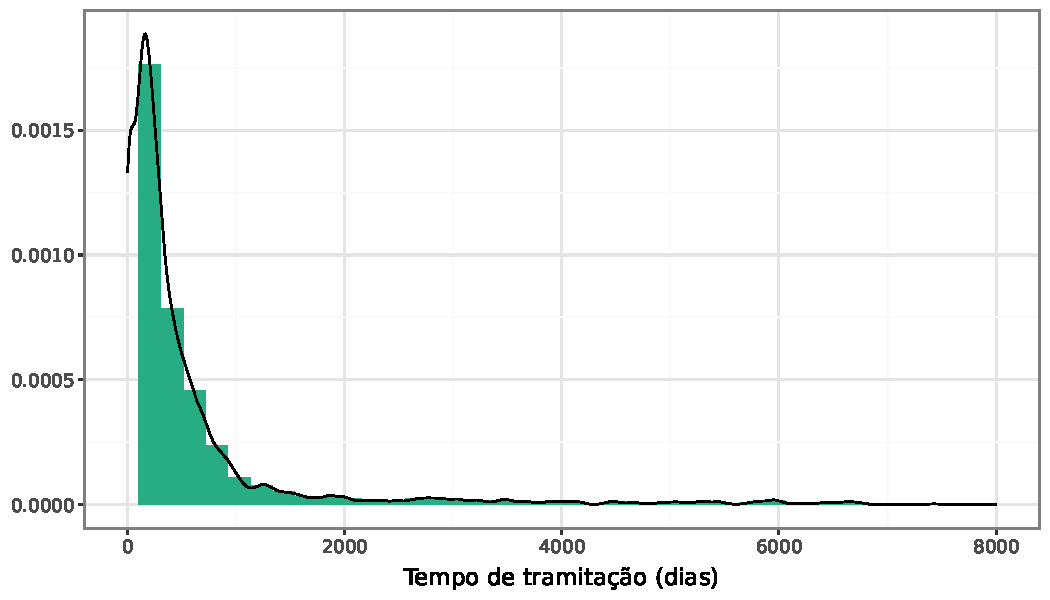
\includegraphics[scale=.85]{imagens/dist_tempo.pdf}
\end{figure}

Dado que se trata do tempo entre uma situação e outra posterior à primeira, todos os valores observados são não-negativos. A maior parte dos processos leva até 2.000 dias para receber baixa. 

A distribuição dos tempos é assimétrica à direita, quase que rigorosamente decrescente. Esse comportamento, por sua vez, não se assemelha ao comportamento de uma distribuição normal, que é simétrica e possui valores negativos com probabilidade não-nula.

Devido à quantidade excessiva de observações, foram feitas 10 amostras aleatórias simples de tamanho 500 sem reposição, e aplicado, para cada, o teste de normalidade de Shapiro-Wilk sob nível de significância de 5\%. As hipóteses foram:

$\begin{cases}
H_{0}: \mbox{O tempo até a baixa segue distribuição Normal.} \\
H_{1}: \mbox{O tempo até a baixa não segue distribuição Normal.}  \\
\end{cases}
$\\

\begin{table}[H]
\centering
\caption{Teste de normalidade de Shapiro-Wilk para amostras do tempo até a baixa}
\begin{tabular}{ccc}
\hline
\textbf{Variáveis} & \textbf{P-valor máximo} & \textbf{Decisão do teste} \\ \hline
Tempo até a baixa & $\approx 0$   & Rejeita $H_0$  \\ \hline  
\end{tabular}
\label{teste:normalidade_tempo}
\end{table}

A Tabela \ref{teste:normalidade_tempo} mostra que mesmo o maior p-valor obtido ainda foi próximo de zero. Para todos os testes, a hipótese de normalidade do tempo até a baixa de um processo foi rejeitada, apresentando, assim, evidências de que sua distribuição não é normal.


\subsubsection{Formato dos processos}
O Conselho Nacional de Justiça instituiu o Processo Judicial Eletrônico (PJe) como forma de tornar o Poder Judiciário mais célere \cite{pje}. A comparação entre os formatos de processos é relevante, não só pela predição do tempo até a baixa, mas também para observar se os resultados da instituição do PJe correspondem aos esperados pelas instituições de justiça.

Espera-se que a quantidade de casos novos físicos diminua progressivamente ao longo do tempo, até se aproximar de zero. A Figura \ref{fig:pct_fisicos_tempo} mostra essa evolução de janeiro 2021 até janeiro de 2024.

\begin{figure}[H]
    \centering
    \caption{Evolução da frequência relativa de casos novos físicos ao longo do tempo}
    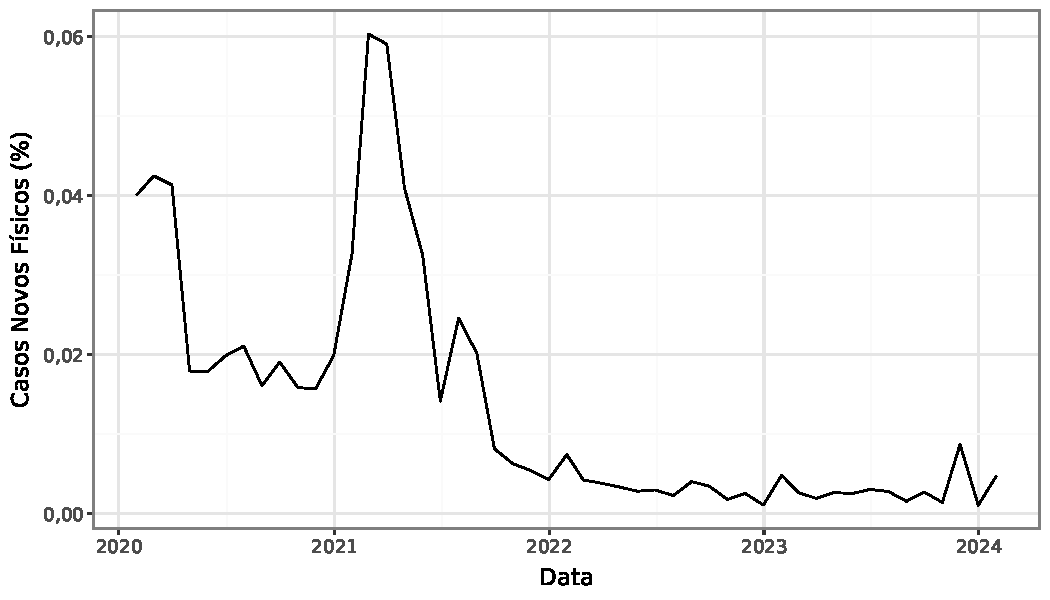
\includegraphics[scale=.87]{imagens/pct_fisicos_tempo.pdf}
    \label{fig:pct_fisicos_tempo}
\end{figure}

A Figura \ref{fig:pct_fisicos_tempo} mostra uma tendência geral de queda. A frequência relativa de casos novos físicos já era de apenas 0,06\% em 2021, e seguiu em queda, chegando a valores muito próximos de zero no começo de 2024.

A Figura \ref{fig:pct_fisicos_tramitando_tempo} mostra a evolução da frequência de processos físicos pendentes tramitando ao longo dos últimos anos.

\begin{figure}[H]
    \centering
    \caption{Evolução da frequência relativa de processos pendentes tramitando em formato físico ao longo do tempo}
    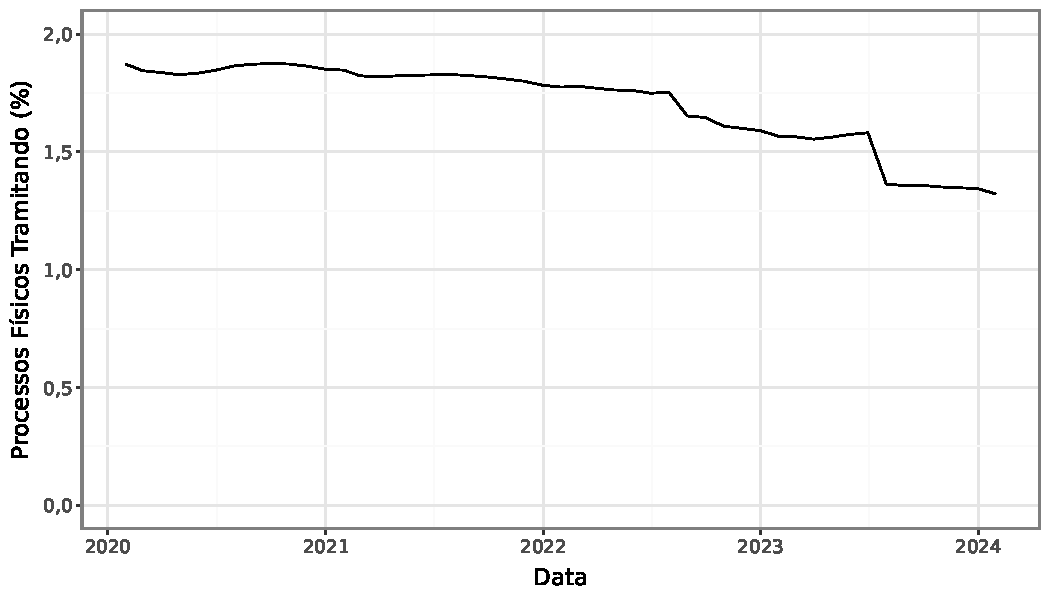
\includegraphics[scale=.85]{imagens/pct_fisicos_tramitando_tempo.pdf}
    \label{fig:pct_fisicos_tramitando_tempo}
\end{figure}

A frequência de processos físicos tramitando permanece relativamente estável e acima de 1\%, apesar de o número de casos novos físicos cair em ritmo acelerado. A discrepância mostra que a maior parte destes processos eletrônicos pendentes não foi iniciada durante o período, sugerindo que os processos com formato físico podem chegar a durar vários anos. A baixa frequência de processos físicos em tramitação também indica que essa variável se trata de um fenômeno raro, em especial durante o período.

A Figura \ref{fig:formato_tempo} mostra a distribuição dos tempos entre o início do processo e a data de referência para cada um dos formatos, onde há processos ainda ativos. Foram omitidos quaisquer processos para os quais o formato era indisponível.

\begin{figure}[H]
    \centering
    \caption{Distribuição dos tempos de tramitação dos processos para cada formato em processos ainda ativos}
    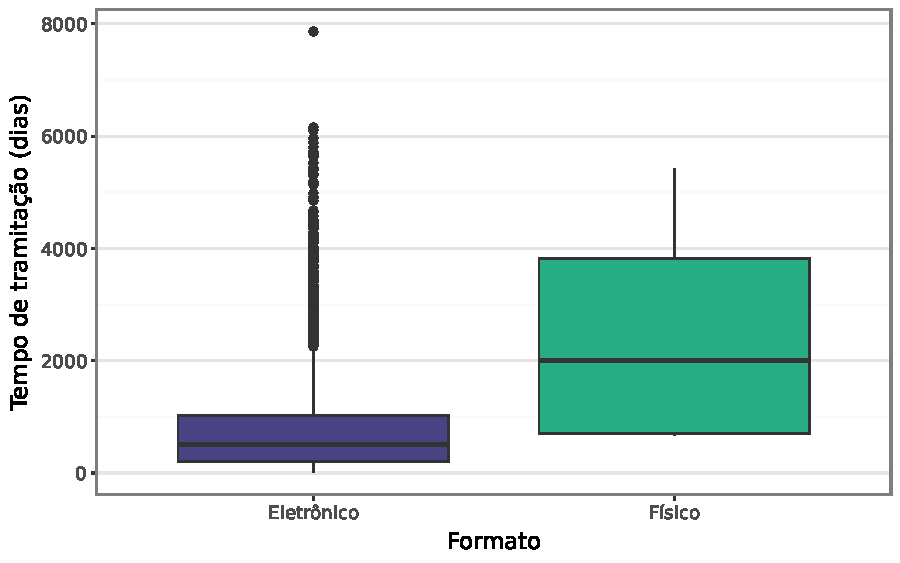
\includegraphics[scale=.93]{imagens/formato_tempo.pdf}
    \label{fig:formato_tempo}
\end{figure}

A Figura \ref{fig:formato_tempo} mostra uma discrepância grande de magnitude entre os tempos de processos físicos e eletrônicos. Cerca de 50\% dos processos físicos tramitando possuem tempo de tramitação próxima ou maior que seis anos.

Além da clara diferença no tempo entre os formatos, há uma variabilidade muito menor dos processos eletrônicos em relação aos processos físicos, que indica que os processos eletrônicos podem ter predições mais precisas.

A diferença sugere que o PJe, de fato, tornou os processos mais céleres, conforme as expectativas do Conselho Nacional de Justiça.


\subsubsection{Graus de jurisdição\label{sec:graus}}
O Poder Judiciário é hierarquizado por três graus de jurisdição: o Primeiro Grau, o Segundo Grau e os Tribunais Superiores. O Primeiro Grau, por sua vez, é também o grau com maior carga processual, fato que motivou a instauração da Política Nacional de Priorização do Primeiro Grau, equilibrando orçamento e pessoal entre os graus segundo suas demandas \cite{justicaemnumeros}.

A Figura \ref{fig:grau_tempo} mostra a distribuição dos tempos até a baixa para o primeiro e segundo graus de jurisdição. Foi feito um corte no eixo Y para evitar que os outliers prejudiquem a visualização.

\begin{figure}[H]
    \centering
    \caption{Distribuição dos tempos até a baixa dos processos para o primeiro e o segundo graus de jurisdição}
    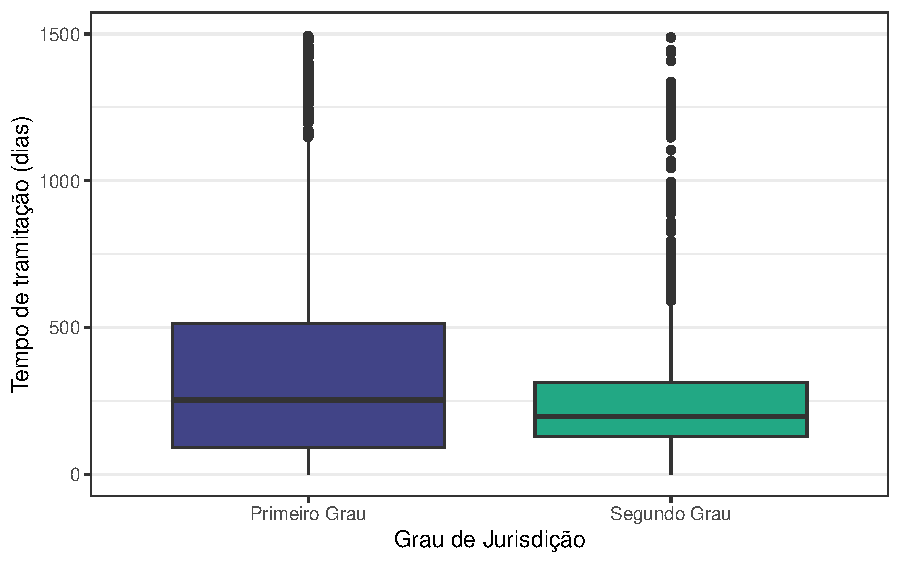
\includegraphics[scale=1]{imagens/grau_tempo.pdf}
    \label{fig:grau_tempo}
\end{figure}

Os tempos até a baixa de um processo são consistentemente menores para o segundo grau, quando comparados com o primeiro. De fato, a discrepância que o Relatório Justiça em Números aponta entre o Primeiro Grau e os outros graus de jurisdição ainda é refletida nos indicadores, tornando o grau uma variável candidata relevante para a predição dos tempos.

\subsubsection{Recursos\label{sec:recursos}}
A primeira decisão judicial sobre um processo é tomada em sua competência originária. Em caso de impugnação de alguma das partes envolvidas no processo, é aberto um recurso para revisar a decisão. O eixo Y foi cortado para evitar prejuízo à visualização devido aos outliers.

\begin{figure}[H]
    \centering
    \caption{Distribuição dos tempos até a baixa dos processos originários e recursais}
   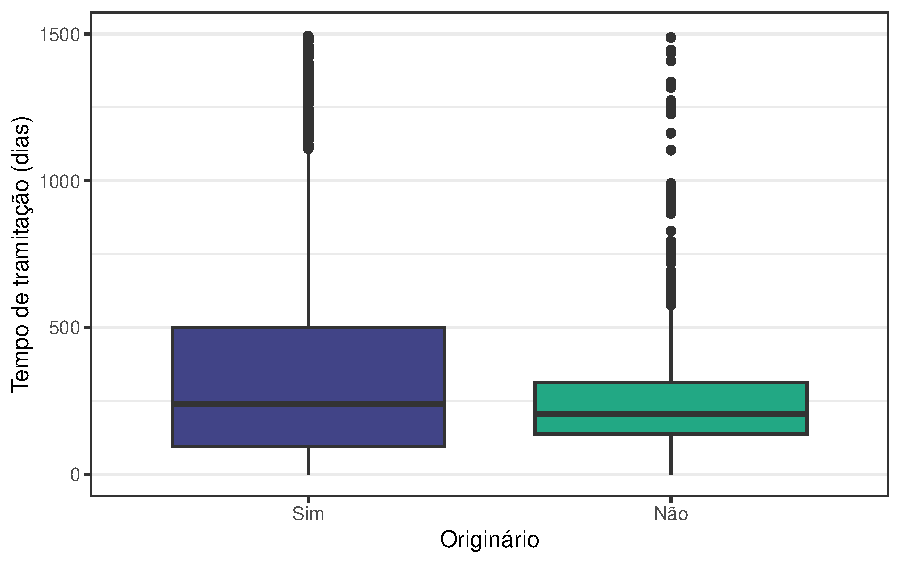
\includegraphics[scale=1]{imagens/originario.pdf}
    \label{fig:originario}
\end{figure}

A Figura \ref{fig:originario} mostra uma diferença de dispersão e de magnitude, onde não só os recursos são mais céleres, como também são concentrados em um intervalo menor.

Ainda, o comportamento dos processos originários e recursais é muito parecido com o comportamento dos processos de primeiro e segundo grau, o que pode indicar associação entre as variáveis. Essa possível associação será discutida na Seção \ref{sec:associacoes_vars}.


\subsubsection{Associação entre as variáveis qualitativas\label{sec:associacoes_vars}}
Foi observada uma semelhança entre os tempos até a baixa nos gráficos da Seção \ref{sec:recursos} e a Seção \ref{sec:graus}.  A Tabela \ref{tbl:originario_grau} investiga as frequências cruzadas de ocorrências de cada grau e nível de recurso.

\begin{table}[H]
\centering
\caption{Frequência de processos pendentes cruzada por grau e recursos}
\begin{tabular}{c|cc|c}
\hline
\multirow{2}{*}{\textbf{Grau}} & \multicolumn{2}{c|}{\textbf{Originário}} & \multirow{2}{*}{\textbf{Total}} \\ 
\cline{2-3}
 & Sim & Não \\ 
  \hline
1º & 5.284.459 &   0  & 5.284.459 \\ 
2º & 113.080 & 670.461 & 783.541 \\ 
   \hline
  Total & 5.397.539 & 670.461 & 6.068.000 \\ 
\hline
\end{tabular}
\label{tbl:originario_grau}
\end{table}

Olhando através dos níveis de recurso, é perceptível que a maior parte das ocorrências originários está compreendida em primeiro grau, bem como a maior parte das ocorrências não-originárias está compreendida em segundo grau. Dentre os processos de segundo grau, há cerca de seis vezes mais processos recursais do que processos originários, e nenhum dos processos recursais observados no período pertence ao primeiro grau.

Visando investigar possíveis outras associações, serão aplicados testes de associação entre as variáveis qualitativas. A Tabela \ref{tbl:assoc_categoricas} exibe o resultado dos testes bivariados de independência para procedimento, grau, originário e formato.

O teste exato de Fisher foi aplicado em todas as tabelas 2x2. Para as tabelas com dimensão maior, foi utilizado o teste Qui-Quadrado de independência.

\begin{table}[H]
\centering
\caption{Testes para Independência entre Variáveis Categóricas}
\begin{tabular}{|cccc|}
\hline
\textbf{Teste} & \textbf{Variáveis} & \textbf{P-valor} & \textbf{Decisão do teste} \\ \hline
Qui-Quadrado & Grau x Procedimento & $\approx 0$   & Rejeita $H_0$  \\ \hline 
Qui-Quadrado & Procedimento x Originário & $\approx 0$   & Não rejeita $H_0$  \\ \hline  
Qui-Quadrado & Procedimento x Formato & 0,628   & Não rejeita $H_0$  \\ \hline
Exato de Fisher & Formato x Grau & 0,307 & Não rejeita $H_0$  \\ \hline
Exato de Fisher & Formato x Originário & 0,585 & Não rejeita $H_0$  \\ \hline
Exato de Fisher & Grau x Originário & $\approx 0$   & Rejeita $H_0$  \\ \hline 
\end{tabular}
\label{tbl:assoc_categoricas}
\end{table}

Não há evidências de que a informação sobre o procedimento esteja associada ao processo ser físico ou eletrônico. Apesar disso, a hipótese de independência foi rejeitada entre procedimento e grau, bem como em procedimento e originário. O teste também confirma o que era apontado pela Tabela \ref{tbl:originario_grau}, mostrando evidências de associação entre grau e originário. Para as outras variáveis, não foram encontradas evidências significativas de associação.


\subsubsection{Procedimentos}
\begin{figure}[H]
    \centering
    \caption{Distribuição dos tempos até a baixa dos processos segundo o procedimento}
    \label{fig:procedimentos_tempo}
    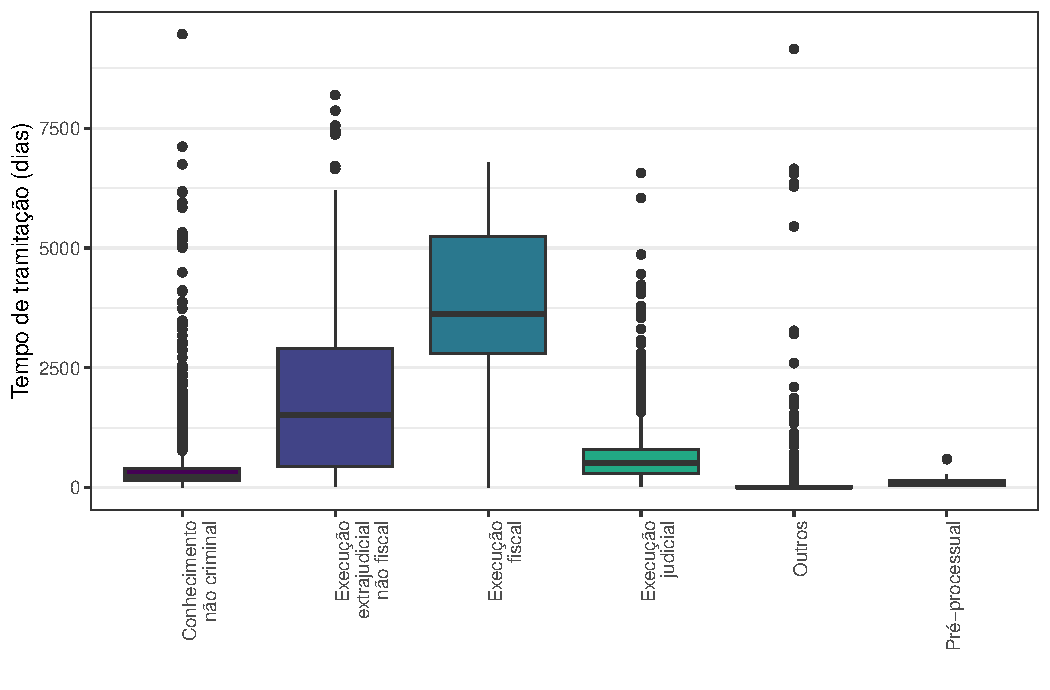
\includegraphics[scale=.9]{imagens/procedimento_tempo.pdf}
\end{figure}

É notável que os procedimentos de conhecimento tendem a apresentar tempos drasticamente menores que os procedimentos de execução. Os pré-processuais e outros, que apresentaram as menores tendências de tempo entre todos os procedimentos observados.

Além da diferença quantitativa entre as execuções, cada execução apresentou um padrão diferente de dispersão. A execução judicial foi a que menos variou entre os três procedimentos de execução. A execução fiscal não apresentou nenhum outlier e teve o maior valor mediano dentre todos os procedimentos, além de apresentar comportamento assimétrico.

\subsubsection{Indicadores quantitativos}
Dos 26 indicadores presentes na Tabela Fato, alguns são correlacionados com outras métricas de forma direta \cite{painelestatistica}. Estão entre eles:
\begin{itemize}
    \item Total de processos Conclusos para o Magistrado a mais de 50 dias: Está correlacionado com o indicador de Conclusos para o Magistrado.
    \item Processos sem tramitação há mais de 50 dias: Está correlacionado ao indicador de Tramitando.
    \item 5\% mais antigos em tramitação: Corresponde a 5\% dos processos no indicador de Tramitando.
    \item Tramitando (ou Pendentes líquidos): Agrega todos os processos que não receberam Baixa, Suspensão ou Sobrestamento.
    \item Pendentes: Agregam todos os processos que não receberam Baixa, incluindo Tramitando, Suspensos e Sobrestados.
    \item Conclusos: Agrega Conclusos para Julgamento, para Despacho, para Admissibilidade recursal, para Decisão, sem especificação e outros.
    \item Audiências: Agrega Audiências Conciliatórias e Não Conciliatórias.
\end{itemize}

Em decorrência das correlações, serão escolhidas as métricas que, sozinhas, agregam a maior quantidade de outros indicadores. A exceção a essa regra será o indicador da situação Tramitando, pois, apesar de estar contido entre os Pendentes, a variável resposta (tempo até a baixa) marca o tempo até a primeira situação de Baixa entre os processos com a situação de Tramitando. Assim sendo, os indicadores são: Tramitando, Suspensos e Sobrestados, Conclusos, Julgamentos, Despachos, Decisões, Audiências, Total de liminares deferidas, Total de liminares indeferidas, Casos Novos de Recurso Interno, Recurso Interno Pendente e Recurso Interno Julgado. A Figura \ref{fig:inds_qtd} mostra a quantidade de ocorrências de cada um dos indicadores selecionados. Apesar de o indicador Pendentes não ter sido incluído, a informação completa dele está incluída, uma vez que os Pendentes são a soma de Tramitando, Suspensos e Sobrestados.

\begin{figure}[H]
    \centering
    \caption{Quantidade de ocorrências em cada métrica}
    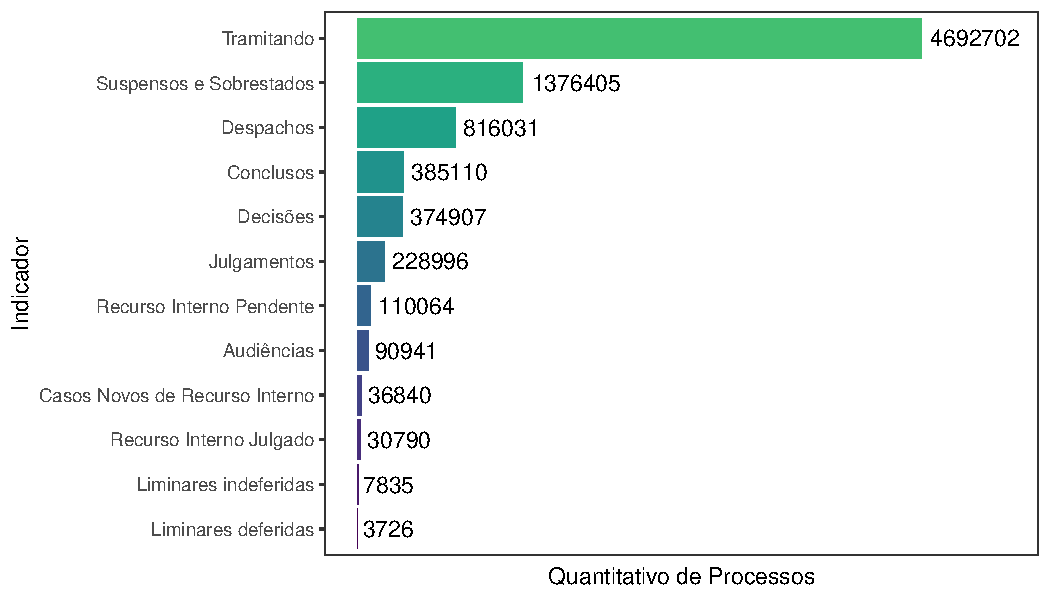
\includegraphics[scale=.9]{imagens/inds_qtd.pdf}
    \label{fig:inds_qtd}
\end{figure}

A quantidade de processos tramitando é a predominante dentre todos os indicadores exibidos. Nos dois indicadores mais frequentes, há um salto entre o primeiro e o segundo, onde o quantitativo de processos tramitando é mais de três vezes superior ao número de suspensos e sobrestados.

Os demais indicadores decaem com poucos saltos, onde os indicadores com menor representação são os de liminares indeferidas e liminares deferidas. Estes, por sua vez, têm uma quantidade de processos pouco maior do que a quantidade de órgãos julgadores. Nota-se que a quantidade de liminares deferidas tem uma média de pouco mais de 1,5 liminares para cada órgão julgador.


A Figura \ref{fig:corr_matrix} investiga possíveis correlações das variáveis explicativas entre elas. 
\begin{figure}[H]
    \centering
    \caption{Matriz de correlações entre as variáveis explicativas}
    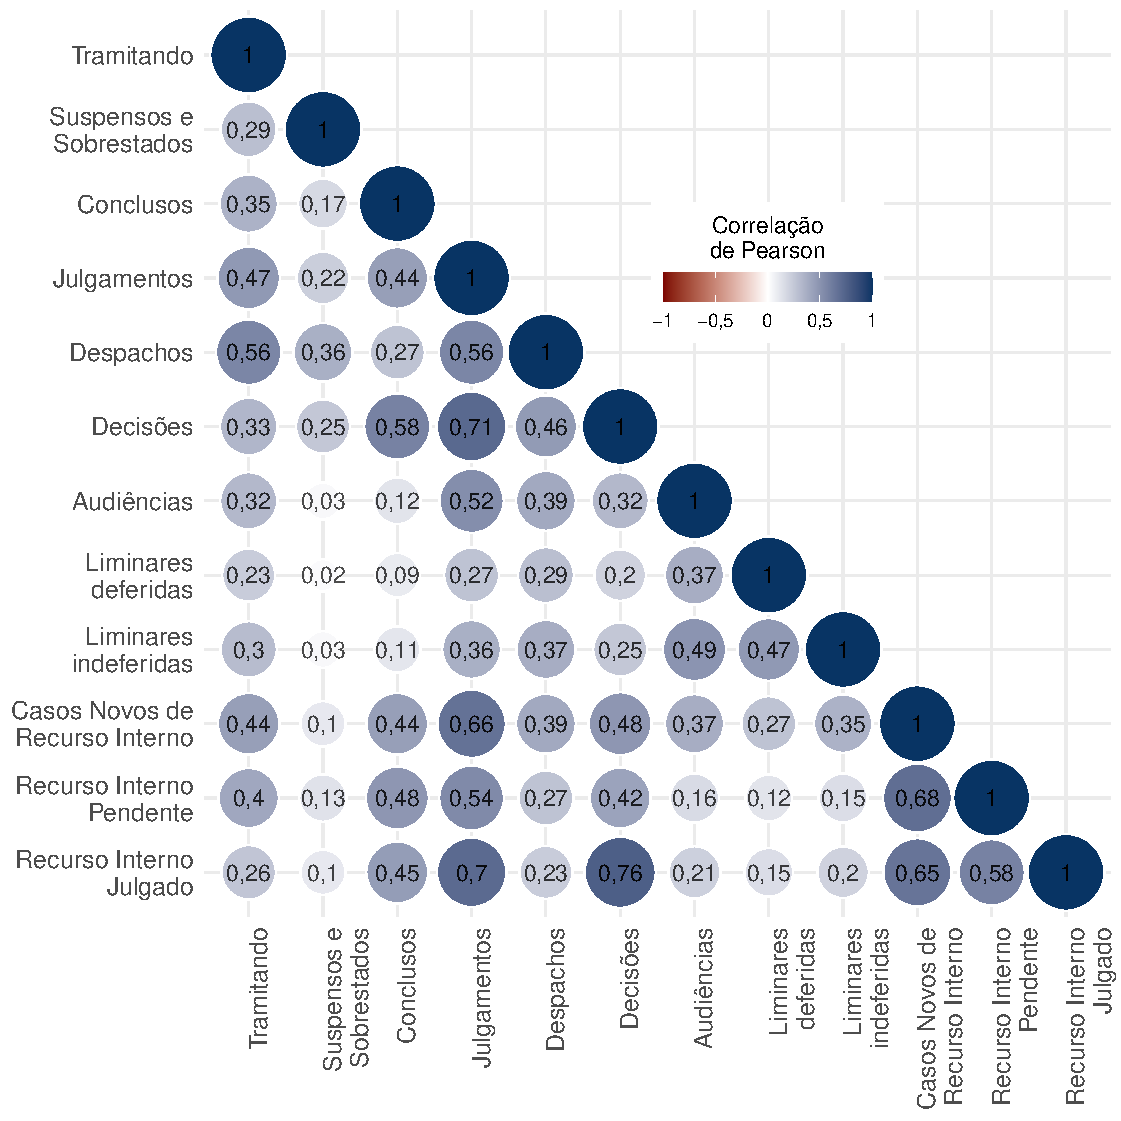
\includegraphics[scale=0.8]{imagens/corrplot.pdf}
    \label{fig:corr_matrix}
\end{figure}

Não houve nenhuma correlação negativa dentre todas as observadas na matriz, embora haja diversas correlações muito próximas de zero.

Os Casos Novos de Recurso Interno, Recurso Interno Pendente e Recurso Interno Julgado, apesar de não conterem um ao outro (como é o caso de outras variáveis supracitadas), não só se correlacionam pelo fato de tratarem de fenômenos relacionados aos recursos internos, como apresentam uma correlação de moderada a forte (aproximadamente de 0,6), com intensidade próxima para todos eles. O indicador Recurso Interno Julgado apresenta uma correlação ainda mais forte com as variáveis Decisões e Julgamentos, que configuraram, também, as maiores correlações observadas na matriz.

As Decisões e Julgamentos, por sua vez, também estão correlacionadas entre elas com intensidade próxima à de Recursos Internos Julgados. Houve uma intensidade moderada entre os dois indicadores e o quantitativo de Conclusos.

Os dois indicadores de Liminares (deferidas e indeferidas), Audiências, Despachos, Conclusos, Suspensos e Sobrestados, não mostraram correlações fortes com nenhum indicador. Os maiores valores registrados para a correlação das liminares indeferidas foram 0,49 e 0,47, com, respectivamente, as variáveis de Audiências e Liminares deferidas. Os outros indicadores citados, eventualmente, apresentaram correlações moderadas entre eles, onde os Conclusos tiveram a maior de suas correlações com as Decisões e os Despachos tiveram suas maiores correlações com Tramitando e Julgamentos.

O indicador Tramitando, mesmo com maior representatividade dentre todos os indicadores, não apresentou correlação forte com nenhum deles, tendo variado entre fraca e moderada.

Os Suspensos e Sobrestados foram os casos que apresentaram menores correlações com todos os indicadores, com valores maiores que 0,3 apenas quando correlacionados com os Despachos.

\subsubsection{Tempo até a baixa por indicador}

A Figura \ref{fig:cross_charts} mostra diagramas de dispersão de cada variável explicativa contra o tempo até a baixa dos processos. A reta azul indica a reta de regressão quantílica para a mediana, enquanto a reta verde indica a reta de regressão gaussiana para a média.

\begin{figure}[H]
    \centering
    \caption{Gráficos de dispersão entre as variáveis explicativas e o tempo até a baixa com retas de regressão quantílica (mediana, em azul) e regressão gaussiana (média, em verde)}
    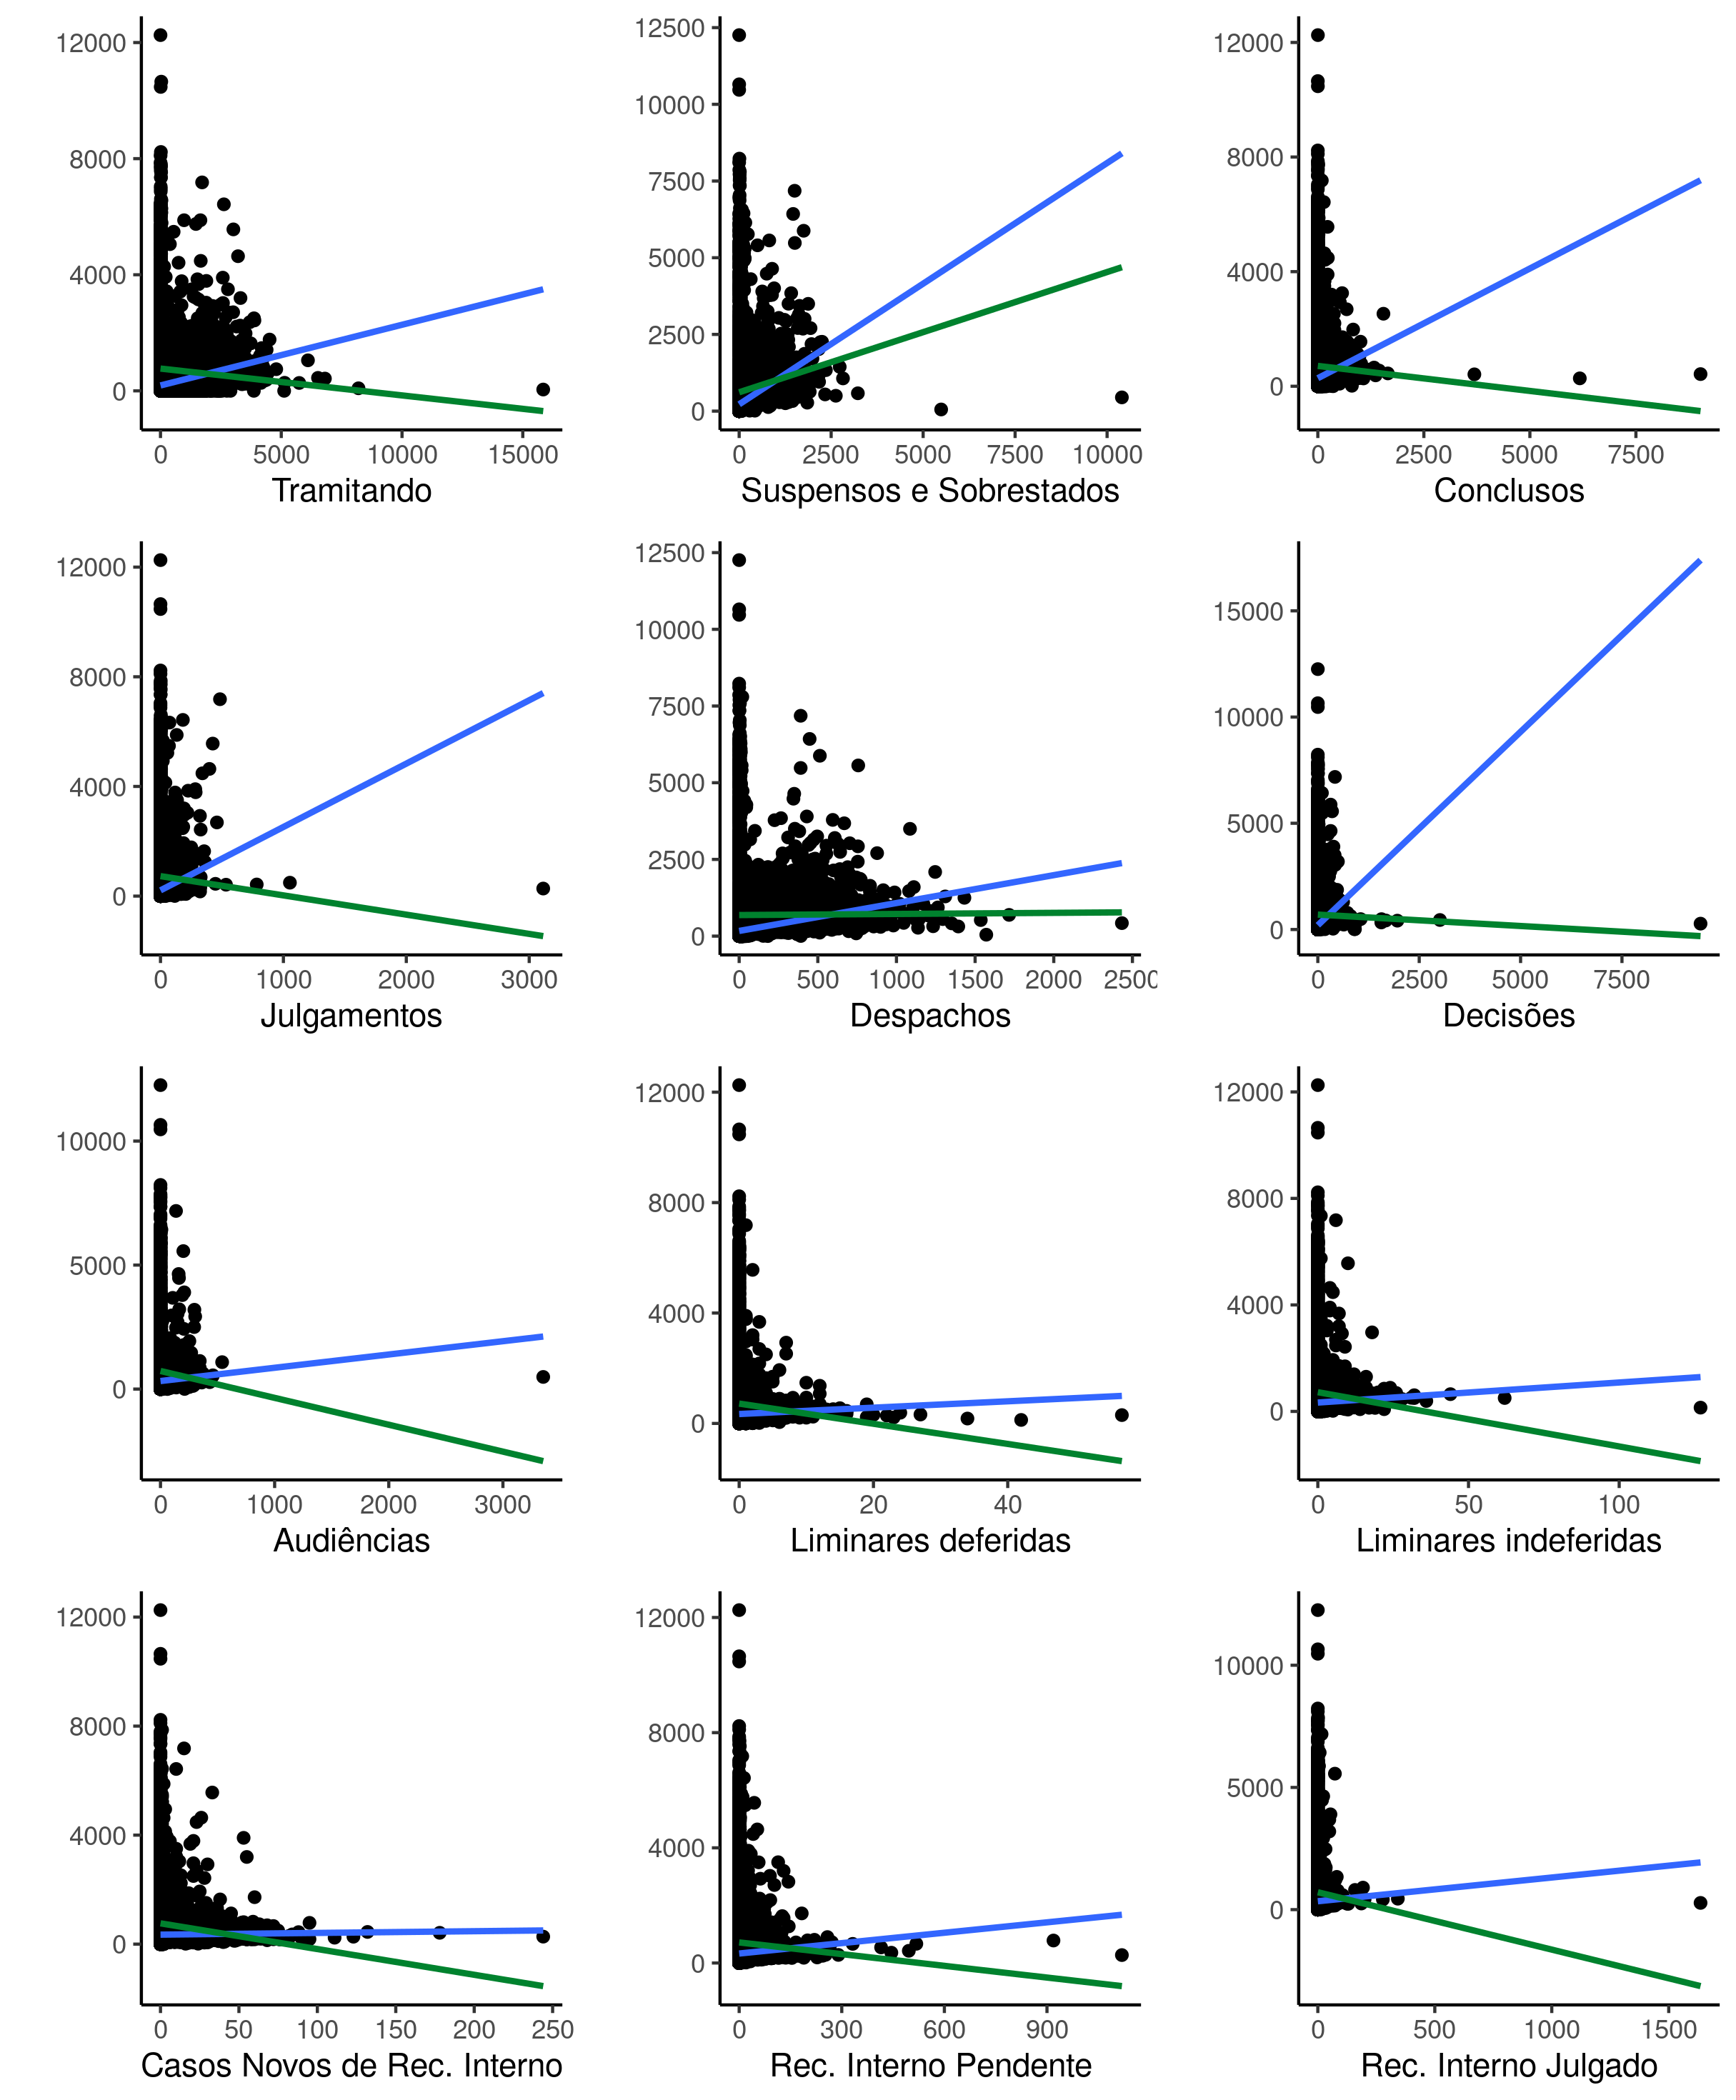
\includegraphics[scale=.745]{imagens/cross_charts.png}
    \label{fig:cross_charts}
\end{figure}

Na visualização bidimensional, não há, segundo os modelos quantílicos, qualquer indicativo de tendência de decrescimento para o tempo mediano de tramitação dos processos conforme o crescimento de um indicador, de modo que esperam-se coeficientes positivos em quaisquer lugares onde eles sejam não-nulos. Apesar disso, vários dos modelos de regressão por mínimos quadrados apresentaram retas decrescentes, eventualmente podendo levar a valores inferiores a zero, sendo eles: Conclusos, julgamentos, decisões, audiências, liminares deferidas, liminares indeferidas, casos novos de recurso interno, recurso interno pendente e recurso interno julgado, de modo que não só a reta mediana e a reta média não coincidem, como se contradizem. Nota-se que a regressão gaussiana é mais suscetível à influência de outliers do que a regressão quantílica.

Apesar de, graficamente, os Casos Novos de Recurso Interno aparentarem ter uma menor inclinação, as inclinações estão prejudicadas não só pela escala do eixo X e Y serem diferentes, como também pela presença de outliers nas variáveis explicativas.

Em todos os indicadores, existe uma concentração grande das observações em torno do valores onde a variável explicativa é próxima de zero. Fica notável a presença de vários órgãos julgadores que, apesar de relatarem poucos processos tramitando, levam um tempo significativamente grande para dar baixa nos processos que existem. A Tabela \ref{tbl:caracteristicas_pendentes_tempo_longo} exibe características das varas com menos de 120 processos pedentes e tempo até a baixa maior que 1.000 dias. 

\begin{table}[ht]
\centering
\caption{Características das varas com menos de 120 processos tramitando e mais de 1.000 dias de tempo até a baixa}
\begin{tabular}{llllrr}
  \hline
  Formato & Grau & Originário & Procedimento & Ocorrências & Tempo \\ 
  \hline
  Eletrônico & 1º & Originário & Execução fiscal & 290 & 4.131 \\ 
  Eletrônico & 1º & Originário & Execução extrajudicial não fiscal & 105 & 3.291 \\ 
  Eletrônico & 2º & Originário & Conhecimento não criminal &  20 & 1.454 \\ 
  Eletrônico & 2º & Recursal & Conhecimento não criminal &  16 & 1.719 \\ 
  Eletrônico & 1º & Originário & Conhecimento não criminal &   7 & 1.394 \\ 
  Eletrônico & 1º & Originário & Outros &   3 & 4.199 \\ 
  Físico &     1º & Originário & Conhecimento não criminal &   3 & 10.936 \\ 
  Eletrônico & 1º & Originário & Execução judicial &   1 & 1.404 \\ 
  Físico &     1º & Originário & Execução judicial &   1 & 2.290 \\ 
   \hline
\end{tabular}
\label{tbl:caracteristicas_pendentes_tempo_longo}
\end{table}

A Tabela \ref{tbl:caracteristicas_pendentes_tempo_longo} mostra que, das varas com menos de 120 processos tramitando e com tempo até a baixa acima de 1.000 dias, 395 (88,56\%) delas estão entre os processos eletrônicos de primeiro grau, originários, com procedimento de execução (fiscal e extrajudicial não fiscal). Esse comportamento está dentro do  esperado, uma vez que, como já observado na Figura \ref{fig:procedimentos_tempo}, os dois procedimentos citados possuem tanto maiores tempos até a baixa quanto maior dispersão nesses tempos, bem como os processos originários e de primeiro grau.

Poucas ocorrências relatavam processos físicos, mas das que relatavam, há três varas com processos físicos cujo tempo até a baixa foi de quase 11.000 dias, que foi o maior valor registrado na tabela. Essas três tinham procedimento de conhecimento não criminal, que foi o único procedimento de conhecimento relatado nos grupos observados, e também o procedimento de conhecimento com maiores tempos até a baixa (Figura \ref{fig:procedimentos_tempo})

A Figura \ref{fig:cross_charts_without_outliers} exibe os mesmos diagramas de dispersão, com a remoção dos outliers tanto das variáveis explicativas e remoção das quatro categorias da tabela \ref{tbl:caracteristicas_pendentes_tempo_longo} que apresentaram os maiores tempos até a baixa. A reta azul indica a reta de regressão quantílica para a mediana, enquanto a reta verde indica a reta de regressão gaussiana para a média.

\begin{figure}[H]
    \centering
    
    \caption{Gráficos de dispersão entre as variáveis explicativas e o tempo até a baixa com retas de regressão quantílica (mediana, em azul) e regressão gaussiana (média, em verde), com remoção de outliers}
    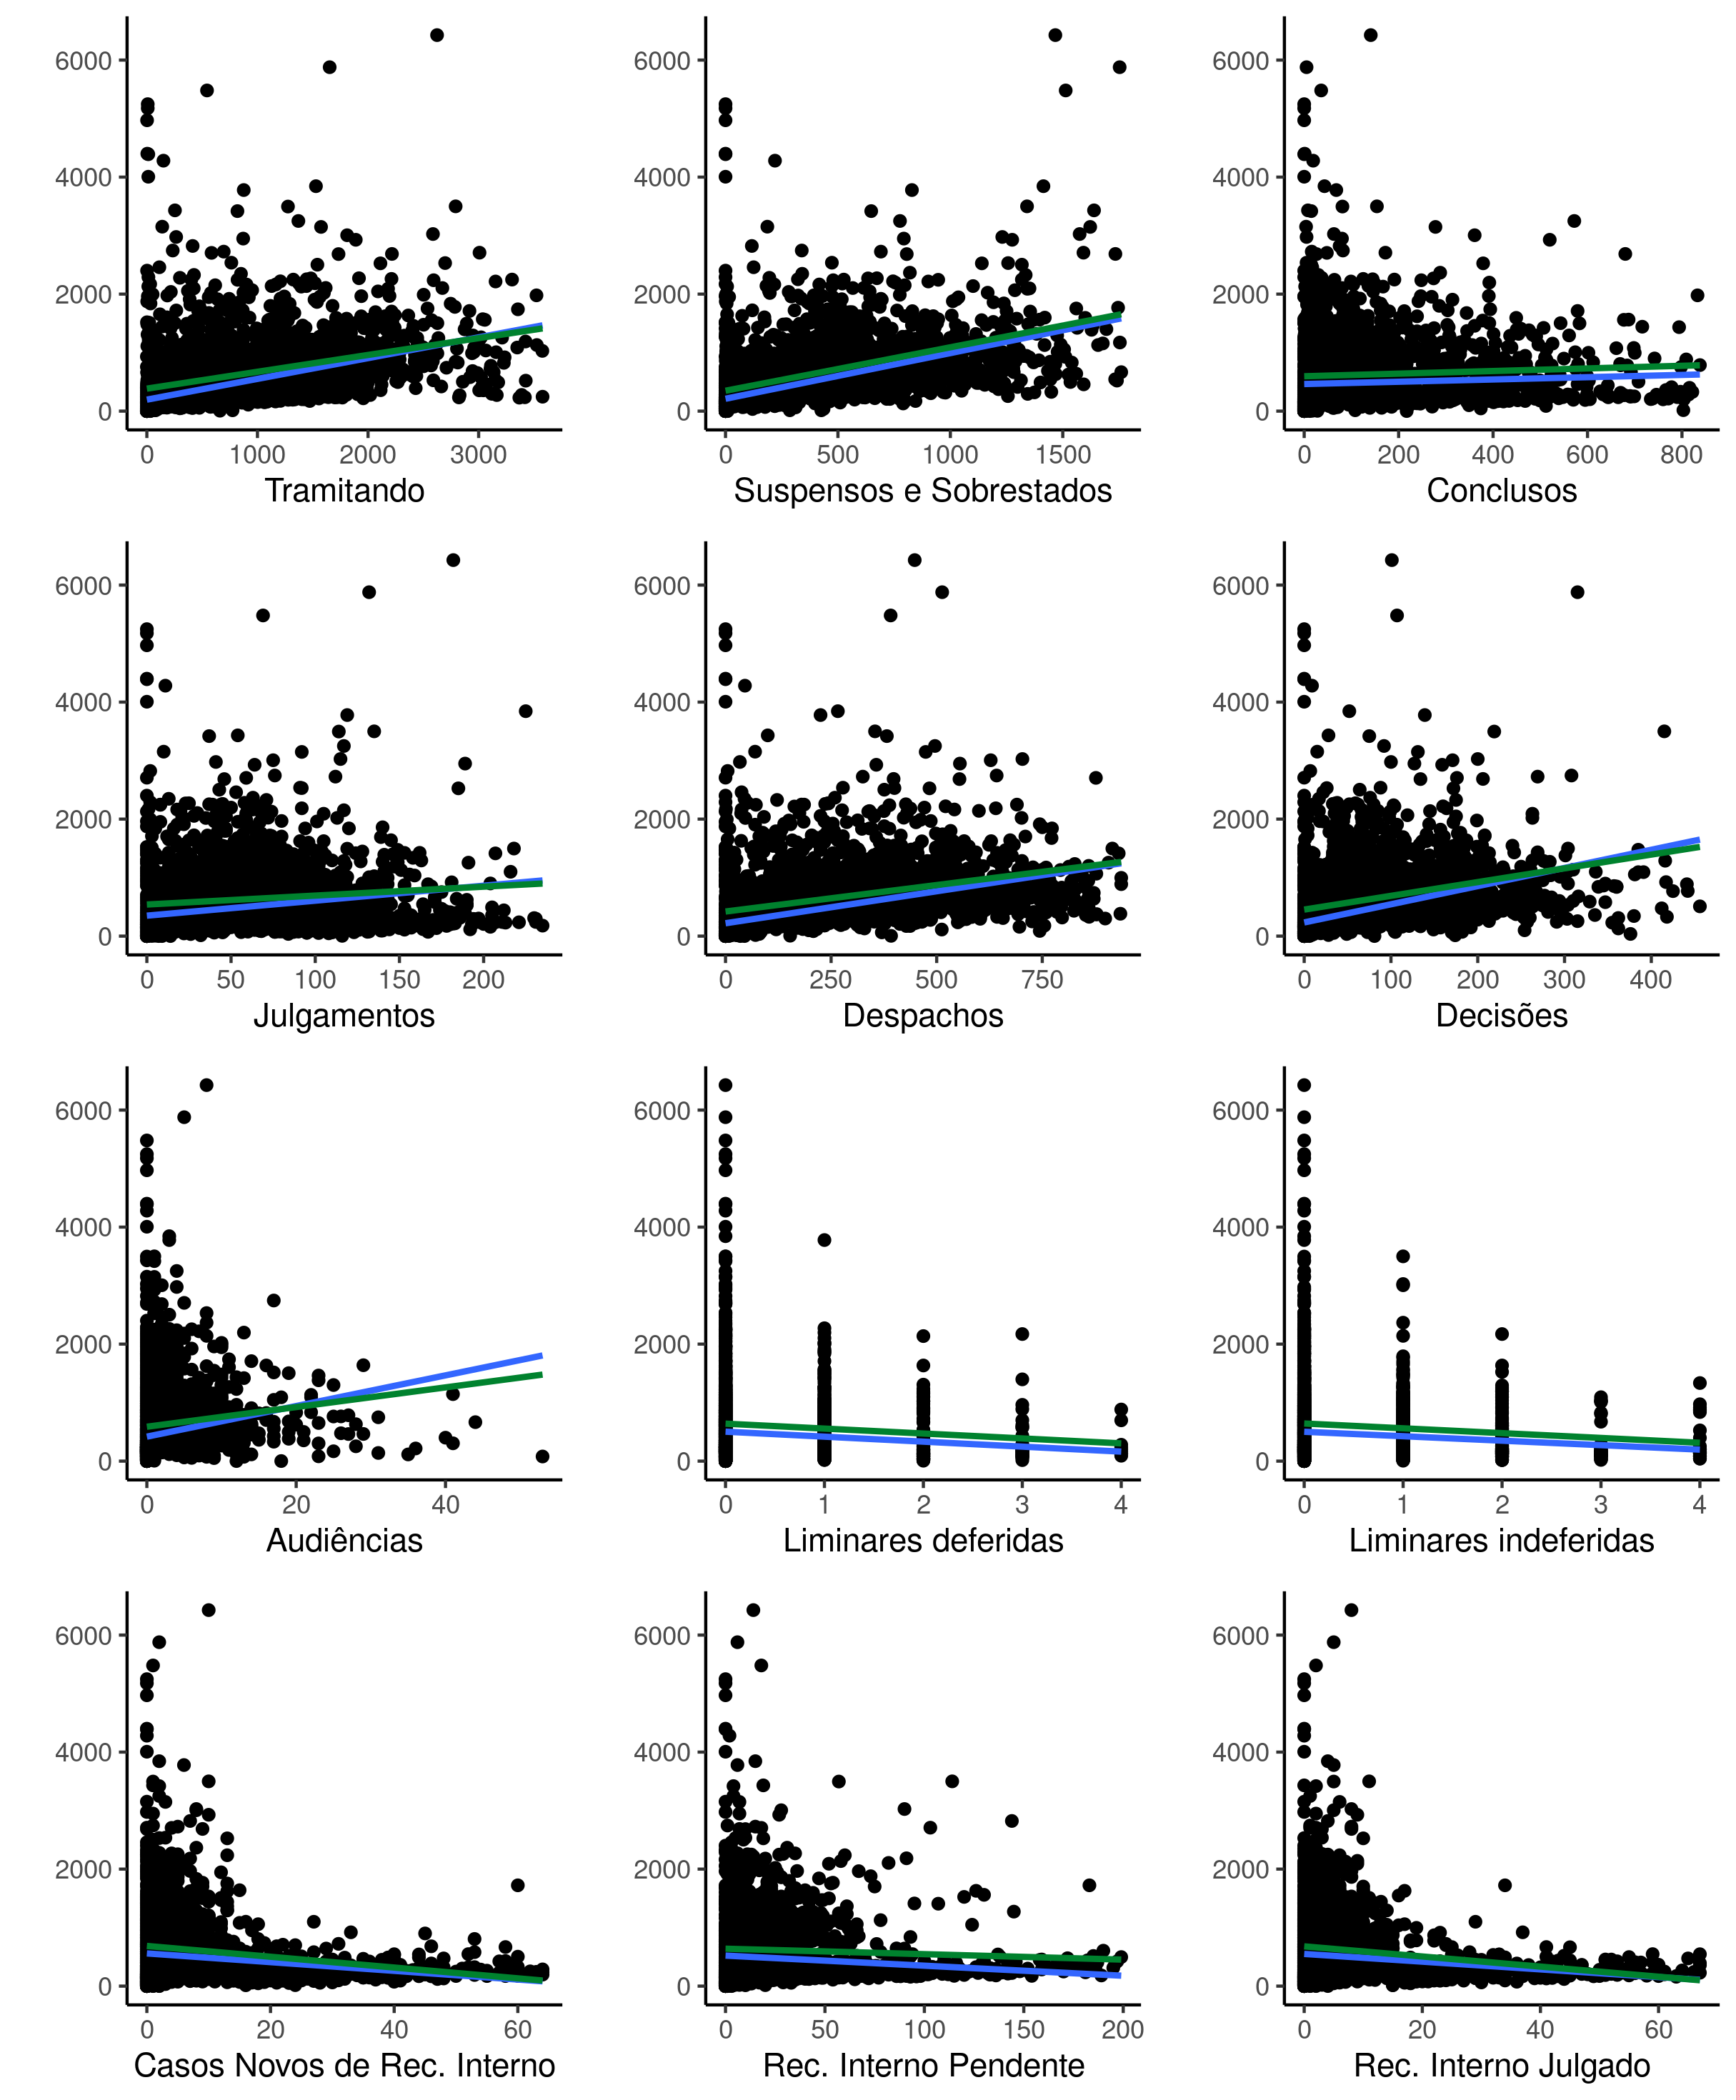
\includegraphics[scale=.74]{imagens/cross_charts_without_outliers.png}
    \label{fig:cross_charts_without_outliers}
\end{figure}

Com a remoção das categorias supracitadas, todas as contradições de tendência entre as médias e as medianas sumiram para todas as variáveis explicativas observadas. Ainda, até mesmo a proximidade das retas aumentou, fornecendo valores, visualmente, muito próximos entre elas.

Outro comportamento que diferiu com a remoção das categorias foi a tendência estritamente crescente da mediana. Agora, as liminares (deferidas e indeferidas), e recursos internos (novos, pendentes e julgados) apresentaram retas medianas decrescentes.

As audiências, liminares e recursos internos ainda apresentam dispersão maior dos tempos até a baixa para valores pequenos das variáveis explicativas, bem como tempos propriamente ditos consideravelmente maiores onde os valores das variáveis explicativas eram próximos de zero. O comportamento delas é não-linear, e elas possuem uma amplitude muito pequena quando comparadas às outras seis variáveis.

\newpage
\subsection{Modelagem}
\subsubsection{Modelos de regressão quantílica sem interações}
Para a construção dos modelos, foram considerados os quantis de nível de 10\%, 25\%, 50\%, 75\% e 90\%.

Os primeiros modelos tiveram a seleção de variáveis baseada unicamente no procedimento automático \textit{stepwise} bidirecional. A Tabela 

\newpage

\section{\textbf{Conclusão}}

A variável Grau e a variável Formato, que já eram variáveis de observância do Conselho Nacional de Justiça no contexto das métricas temporais, como observado na implementação do PJe \cite{pje} e da Política Nacional de Priorização do Primeiro Grau \cite{justicaemnumeros} se mostraram relevantes nos modelos. Em especial, a variável Grau apareceu em todos. O estudo mostrou que a instituição do PJe foi bem-sucedida, reduzindo drasticamente a duração média dos processos. A Justiça do Trabalho, por sua vez, está com quase todo o acervo em ambiente eletrônico. 

O número de processos tramitando se mostrou a variável mais relevante das variáveis quantitativas. Apesar de, individualmente, aumentar poucas horas no tempo médio de duração dos processos, ela foi a única dentre as variáveis quantitativas que apareceu consistentemente em todos os modelos, tanto quantílicos quanto gaussianos.

Verificou-se que as decisões têm influência negativa no tempo, de modo que, quanto mais decisões forem proferidas, menor o tempo esperado até a baixa dos processos. Esse comportamento se repetiu para todos os modelos onde a variável foi incluída. 

O estudo demonstrou que a regressão quantílica apresenta resultados promissores no contexto da estimação de métricas temporais do Poder Judiciário, mostrando não só que essa predição é possível, como que as variáveis disponíveis publicamente são úteis para predizê-las. O método se torna mais relevante pelo fato de que os efeitos de cada variável são diferentes em cada um dos níveis de tempo. O modelo para a mediana, especificamente, foi útil também a nível preditivo, apresentando um erro menor que o modelo gaussiano (mesmo utilizando menos variáveis).

Embora o estudo tenha se restringido à Justiça do Trabalho, modelagens semelhantes podem ser feitas para os outros ramos de justiça, sendo possível investigar a distribuição dos tempos até a baixa para cada ramo. De forma análoga, existem outras variáveis temporais oriundas do DataJud, como tempo médio do pendente líquido e tempo médio até o julgamento, que poderiam ser estudadas através de metodologias semelhantes. Outras variáveis que não estavam disponíveis no mesmo nível de agregação dos dados desse trabalho, como número de servidores e número de juízes e magistrados, permitem construir novas hipóteses e abrem espaço para estudos futuros.
\newpage
%
%\newpage
%
%%\section*{\textbf{Referências}}
%% Inserir as Referências Bibliográficas.




%
%\newpage

\addcontentsline{toc}{section}{\textbf{Referências}}
\bibliographystyle{abntex2-alf}
\bibliography{ref.bib}

%\newpage
%\fancyhead[RE,LO]{\textit{Apêndice}}
%\addcontentsline{toc}{section}{\textbf{Apêndice}}
%\section*{Apêndice}
%\appendix
%\section{nome apêndice 1}
texto...

\section{nome apêndice 2}
texto...
%
%\newpage
%\fancyhead[RE,LO]{\textit{Anexo}}
%\appendix
%\addcontentsline{toc}{section}{\textbf{Anexo}}
%\section*{Anexo}
%
%\section{nome anexo 1}
texto...


\end{document}
